
%-----------------------------------------------------------------------------------------------------------------------------------------------%
%	The MIT License (MIT)
%
%	Copyright (c) 2019 Jan Küster
%
%	Permission is hereby granted, free of charge, to any person obtaining a copy
%	of this software and associated documentation files (the "Software"), to deal
%	in the Software without restriction, including without limitation the rights
%	to use, copy, modify, merge, publish, distribute, sublicense, and/or sell
%	copies of the Software, and to permit persons to whom the Software is
%	furnished to do so, subject to the following conditions:
%	
%	THE SOFTWARE IS PROVIDED "AS IS", WITHOUT WARRANTY OF ANY KIND, EXPRESS OR
%	IMPLIED, INCLUDING BUT NOT LIMITED TO THE WARRANTIES OF MERCHANTABILITY,
%	FITNESS FOR A PARTICULAR PURPOSE AND NONINFRINGEMENT. IN NO EVENT SHALL THE
%	AUTHORS OR COPYRIGHT HOLDERS BE LIABLE FOR ANY CLAIM, DAMAGES OR OTHER
%	LIABILITY, WHETHER IN AN ACTION OF CONTRACT, TORT OR OTHERWISE, ARISING FROM,
%	OUT OF OR IN CONNECTION WITH THE SOFTWARE OR THE USE OR OTHER DEALINGS IN
%	THE SOFTWARE.
%	
%
%-----------------------------------------------------------------------------------------------------------------------------------------------%


%============================================================================%
%
%	DOCUMENT DEFINITION
%
%============================================================================%

\documentclass[3pt,A4,english]{article}	


%----------------------------------------------------------------------------------------
%	ENCODING
%----------------------------------------------------------------------------------------

% we use utf8 since we want to build from any machine
\usepackage[utf8]{inputenc}		
\usepackage[USenglish]{isodate}
\usepackage{fancyhdr}
% \usepackage[numbers]{natbib}

%----------------------------------------------------------------------------------------
%	LOGIC
%----------------------------------------------------------------------------------------
\def\labelitemi{}

% provides \isempty test
\usepackage{xstring, xifthen}
\usepackage{enumitem}
\setlist[itemize]{nosep, leftmargin=0.5em, itemsep=0.5em, before=\fontsize{9}{12}\selectfont } % Align bullet with first line
\usepackage[english]{babel}
\usepackage{blindtext}
\usepackage{pdfpages}
\usepackage{changepage}
%----------------------------------------------------------------------------------------
%	FONT BASICS
%----------------------------------------------------------------------------------------

% some tex-live fonts - choose your own
\usepackage[default]{raleway}

% set font default
\renewcommand*\familydefault{\sfdefault} 	
\usepackage[T1]{fontenc}

% more font size definitions
\usepackage{moresize}

%----------------------------------------------------------------------------------------
%	FONT AWESOME ICONS
%---------------------------------------------------------------------------------------- 

% include the fontawesome icon set
\usepackage{fontawesome5}

% use to vertically center content
% credits to: http://tex.stackexchange.com/questions/7219/how-to-vertically-center-two-images-next-to-each-other
\newcommand{\vcenteredinclude}[1]{\begingroup
\setbox0=\hbox{\includegraphics{#1}}%
\parbox{\wd0}{\box0}\endgroup}
\newcommand{\tab}[1]{\hspace{.2\textwidth}\rlap{#1}}
% use to vertically center content
% credits to: http://tex.stackexchange.com/questions/7219/how-to-vertically-center-two-images-next-to-each-other
\newcommand*{\vcenteredhbox}[1]{\begingroup
\setbox0=\hbox{#1}\parbox{\wd0}{\box0}\endgroup}

% icon shortcut
\newcommand{\icon}[2] { 							
	\makebox(#2, #2){\textcolor{maincol}{\textcolor{maincol}{\faIcon{#1}}}}
}	


% icon with text shortcut
\newcommand{\icontext}[3]{ 						
	\vcenteredhbox{\icon{#1}{#2}}  \hspace{2pt}  \parbox{0.9\mpwidth}{\textcolor{black}{#3}}
}

% icon with website url
\newcommand{\iconhref}[4]{ 						
    \vcenteredhbox{\icon{#1}{#2}}  \hspace{2pt} \href{#4}{\textcolor{black}{#3}}
}

% icon with email link
\newcommand{\iconemail}[5]{ 						
    \vcenteredhbox{\icon{#1}{#2}{#5}}  \hspace{2pt} \href{mailto:#4}{\textcolor{#5}{#3}}
}

%----------------------------------------------------------------------------------------
%	PAGE LAYOUT  DEFINITIONS
%----------------------------------------------------------------------------------------

% page outer frames (debug-only)
% \usepackage{showframe}		

% we use paracol to display breakable two columns
\usepackage{paracol}
\usepackage{tikzpagenodes}
\usetikzlibrary{calc}
\usepackage{lmodern}
\usepackage{multicol}
\usepackage{lipsum}
\usepackage{atbegshi}
% define page styles using geometry
\usepackage[a4paper]{geometry}

% remove all possible margins
\geometry{top=1cm, bottom=1cm, left=1cm, right=1cm}

\usepackage{fancyhdr}
\pagestyle{empty}

% space between header and content
% \setlength{\headheight}{0pt}

% indentation is zero
\setlength{\parindent}{0mm}

%----------------------------------------------------------------------------------------
%	TABLE /ARRAY DEFINITIONS
%---------------------------------------------------------------------------------------- 

% extended aligning of tabular cells
\usepackage{array}

% custom column right-align with fixed width
% use like p{size} but via x{size}
\newcolumntype{x}[1]{%
>{\raggedleft\hspace{0pt}}p{#1}}%


%----------------------------------------------------------------------------------------
%	GRAPHICS DEFINITIONS
%---------------------------------------------------------------------------------------- 

%for header image
\usepackage{graphicx}

% use this for floating figures
% \usepackage{wrapfig}
% \usepackage{float}
% \floatstyle{boxed} 
% \restylefloat{figure}

%for drawing graphics		
\usepackage{tikz}			
\usepackage{ragged2e}	
\usetikzlibrary{shapes, backgrounds,mindmap, trees}

%----------------------------------------------------------------------------------------
%	Bibliography
%---------------------------------------------------------------------------------------- 

%----------------------------------------------------------------------------------------
%	Color DEFINITIONS
%---------------------------------------------------------------------------------------- 
\usepackage{transparent}
\usepackage{color}

% primary color
\definecolor{maincol}{HTML}{B83B5E}

% accent color, secondary
% \definecolor{accentcol}{RGB}{ 250, 150, 10 }

% dark color
\definecolor{darkcol}{RGB}{ 70, 70, 70 }

% light color
\definecolor{lightcol}{RGB}{245,245,245}

\definecolor{accentcol}{HTML}{6A2C70}






% Package for links, must be the last package used
\usepackage[hidelinks]{hyperref}

% returns minipage width minus two times \fboxsep
% to keep padding included in width calculations
% can also be used for other boxes / environments
\newcommand{\mpwidth}{\linewidth-\fboxsep-\fboxsep}
	


%============================================================================%
%
%	CV COMMANDS
%
%============================================================================%

%----------------------------------------------------------------------------------------
%	 CV LIST
%----------------------------------------------------------------------------------------

% renders a standard latex list but abstracts away the environment definition (begin/end)
\newcommand{\cvlist}[1] {
	\begin{itemize}{#1}\end{itemize}
}

%----------------------------------------------------------------------------------------
%	 CV TEXT
%----------------------------------------------------------------------------------------

% base class to wrap any text based stuff here. Renders like a paragraph.
% Allows complex commands to be passed, too.
% param 1: *any
\newcommand{\cvtext}[1] {
	\begin{tabular*}{1\mpwidth}{p{0.98\mpwidth}}
		\parbox{1\mpwidth}{#1}
	\end{tabular*}
}
\newcommand{\cvtextsmall}[1] {
	\begin{tabular*}{0.8\mpwidth}{p{0.8\mpwidth}}
		\parbox{0.8\mpwidth}{#1}
	\end{tabular*}
}
%----------------------------------------------------------------------------------------
%	CV SECTION
%----------------------------------------------------------------------------------------

% Renders a a CV section headline with a nice underline in main color.
% param 1: section title
\newlength{\barw}
\newcommand{\cvsection}[1] {
	\vspace{10pt}
	\settowidth{\barw}{\textbf{\LARGE #1}}
	\cvtext{
		\textbf{\LARGE{\textcolor{darkcol}{#1}}}\\[-4pt]
		\textcolor{accentcol}{ \rule{\barw}{1.5pt} }
	}
}

\newcommand{\cvsubsection}[1] {
	\vspace{4pt}
	\settowidth{\barw}{\textbf{\Large #1}}
	\cvtext{
		\textbf{\Large{\textcolor{darkcol}{#1}}}\\[-4pt]
		\textcolor{accentcol}{ \rule{\barw}{1.5pt} } \\
	}
}

\newcommand{\cvheadline}[1] {
	\vspace{13pt}
	\cvtext{
		\textbf{\Huge{\textcolor{accentcol}{#1}}}\\[-4pt]
		 
	}
}

\newcommand{\cvsubheadline}[1] {
	\vspace{13pt}
	\cvtext{
		\textbf{\huge{\textcolor{darkcol}{#1}}}\\[-4pt]
		 
	}
}
%----------------------------------------------------------------------------------------
%	META SKILL
%----------------------------------------------------------------------------------------

% Renders a progress-bar to indicate a certain skill in percent.
% param 1: name of the skill / tech / etc.
% param 2: level (for example in years)
% param 3: percent, values range from 0 to 1
\newcommand{\cvskill}[3] {
	\begin{tabular*}{1\mpwidth}{p{0.72\mpwidth}  r}
 		\textcolor{black}{\textbf{#1}} & \textcolor{maincol}{#2}\\
	\end{tabular*}%
	
	\hspace{4pt}
	\begin{tikzpicture}[scale=1,rounded corners=2pt,very thin]
		\fill [lightcol] (0,0) rectangle (1\mpwidth, 0.15);
		\fill [accentcol] (0,0) rectangle (#3\mpwidth, 0.15);
  	\end{tikzpicture}%
}


%----------------------------------------------------------------------------------------
%	 CV EVENT
%----------------------------------------------------------------------------------------

% Renders a table and a paragraph (cvtext) wrapped in a parbox (to ensure minimum content
% is glued together when a pagebreak appears).
% Additional Information can be passed in text or list form (or other environments).
% the work you did
% param 1: time-frame i.e. Sep 14 - Jan 15 etc.
% param 2:	 event name (job position etc.)
% param 3: Customer, Employer, Industry
% param 4: Short description
% param 5: work done (optional)
% param 6: technologies include (optional)
% param 7: achievements (optional)
\newcommand{\cvevent}[3] {
	
	% we wrap this part in a parbox, so title and description are not separated on a pagebreak
	% if you need more control on page breaks, remove the parbox
	\parbox{\mpwidth}{
		\begin{tabular*}{1\mpwidth}{p{0.66\mpwidth}  r}
	 		\textcolor{black}{\textbf{#2}} & \colorbox{accentcol}{\makebox[0.32\mpwidth]{\textcolor{white}{\textbf{#1}}}} \\
			\textcolor{maincol}{#3} & \\
		\end{tabular*}\\[4pt]
	
		% \ifthenelse{\isempty{#4}}{}{
		% 	\cvtext{#4}\\
		% }
	}
	\vspace{0pt}
}



%----------------------------------------------------------------------------------------
%	 CV META EVENT
%----------------------------------------------------------------------------------------

% Renders a CV event on the sidebar
% param 1: title
% param 2: subtitle (optional)
% param 3: customer, employer, etc,. (optional)
% param 4: info text (optional)
\newcommand{\cvmetaevent}[4] {
	\textcolor{maincol} { \cvtext{\textbf{\begin{flushleft}#1\end{flushleft}}}}

	\ifthenelse{\isempty{#2}}{}{
	\textcolor{black} {\cvtext{{#2}} }
	}
	\ifthenelse{\isempty{#3}}{}{
		\cvtext{{ \textcolor{maincol} {#3} }}
	}

	\cvtext{#4}\\[4pt]
}

%---------------------------------------------------------------------------------------
%	QR CODE
%----------------------------------------------------------------------------------------

% Renders a qrcode image (centered, relative to the parentwidth)
% param 1: percent width, from 0 to 1
\newcommand{\cvqrcode}[1] {
	\begin{center}
		\includegraphics[width={#1}\mpwidth]{qrcode}
	\end{center}
}


% HEADER AND FOOOTER 
%====================================
\newcommand\Header[1]{%
\begin{tikzpicture}[remember picture,overlay]
\fill[accentcol]
  (current page.north west) -- (current page.north east) --
  ([yshift=50pt]current page.north east|-current page text area.north east) --
  ([yshift=50pt,xshift=-3cm]current page.north|-current page text area.north) --
  ([yshift=3pt,xshift=-5cm]current page.north|-current page text area.north) --
  ([yshift=3pt]current page.north west|-current page text area.north west) -- cycle;
\node[font=\sffamily\bfseries\color{white},anchor=west,
  xshift=0.7cm,yshift=-0.32cm] at (current page.north west)
  {\fontsize{12}{12}\selectfont {#1}};
\end{tikzpicture}%
}

\newcommand\Footer[1]{%
\begin{tikzpicture}[remember picture,overlay]
\fill[lightcol]
  (current page.south east) -- (current page.south west) --
  ([yshift=-80pt]current page.south east|-current page text area.south east) --
  ([yshift=-80pt,xshift=-6cm]current page.south|-current page text area.south) --
  ([xshift=-2.5cm,yshift=-3pt]current page.south|-current page text area.south) --	
  ([yshift=-3pt]current page.south east|-current page text area.south east) -- cycle;
\node[yshift=0.32cm,xshift=9cm] at (current page.south) {\fontsize{10}{10}\selectfont \textbf{\thepage}};
\end{tikzpicture}%
}


%=====================================
%============================================================================%
%
%
%
%	DOCUMENT CONTENT
%
%
%
%============================================================================%
\begin{document}

\columnratio{0.31}
\setlength{\columnsep}{2.2em}
\setlength{\columnseprule}{4pt}
\colseprulecolor{white}


% LEBENSLAUF HIERE
\AtBeginShipoutFirst{\Header{David Munoz-Tord}\Footer{1}}
\AtBeginShipout{\AtBeginShipoutAddToBox{\Header{David
Munoz-Tord}\Footer{2}}}

\newpage

\colseprulecolor{lightcol}
\columnratio{0.31}
\setlength{\columnsep}{2.2em}
\setlength{\columnseprule}{4pt}
\begin{paracol}{2}
	\begin{leftcolumn}
		%---------------------------------------------------------------------------------------
		%	META IMAGE
		%----------------------------------------------------------------------------------------
		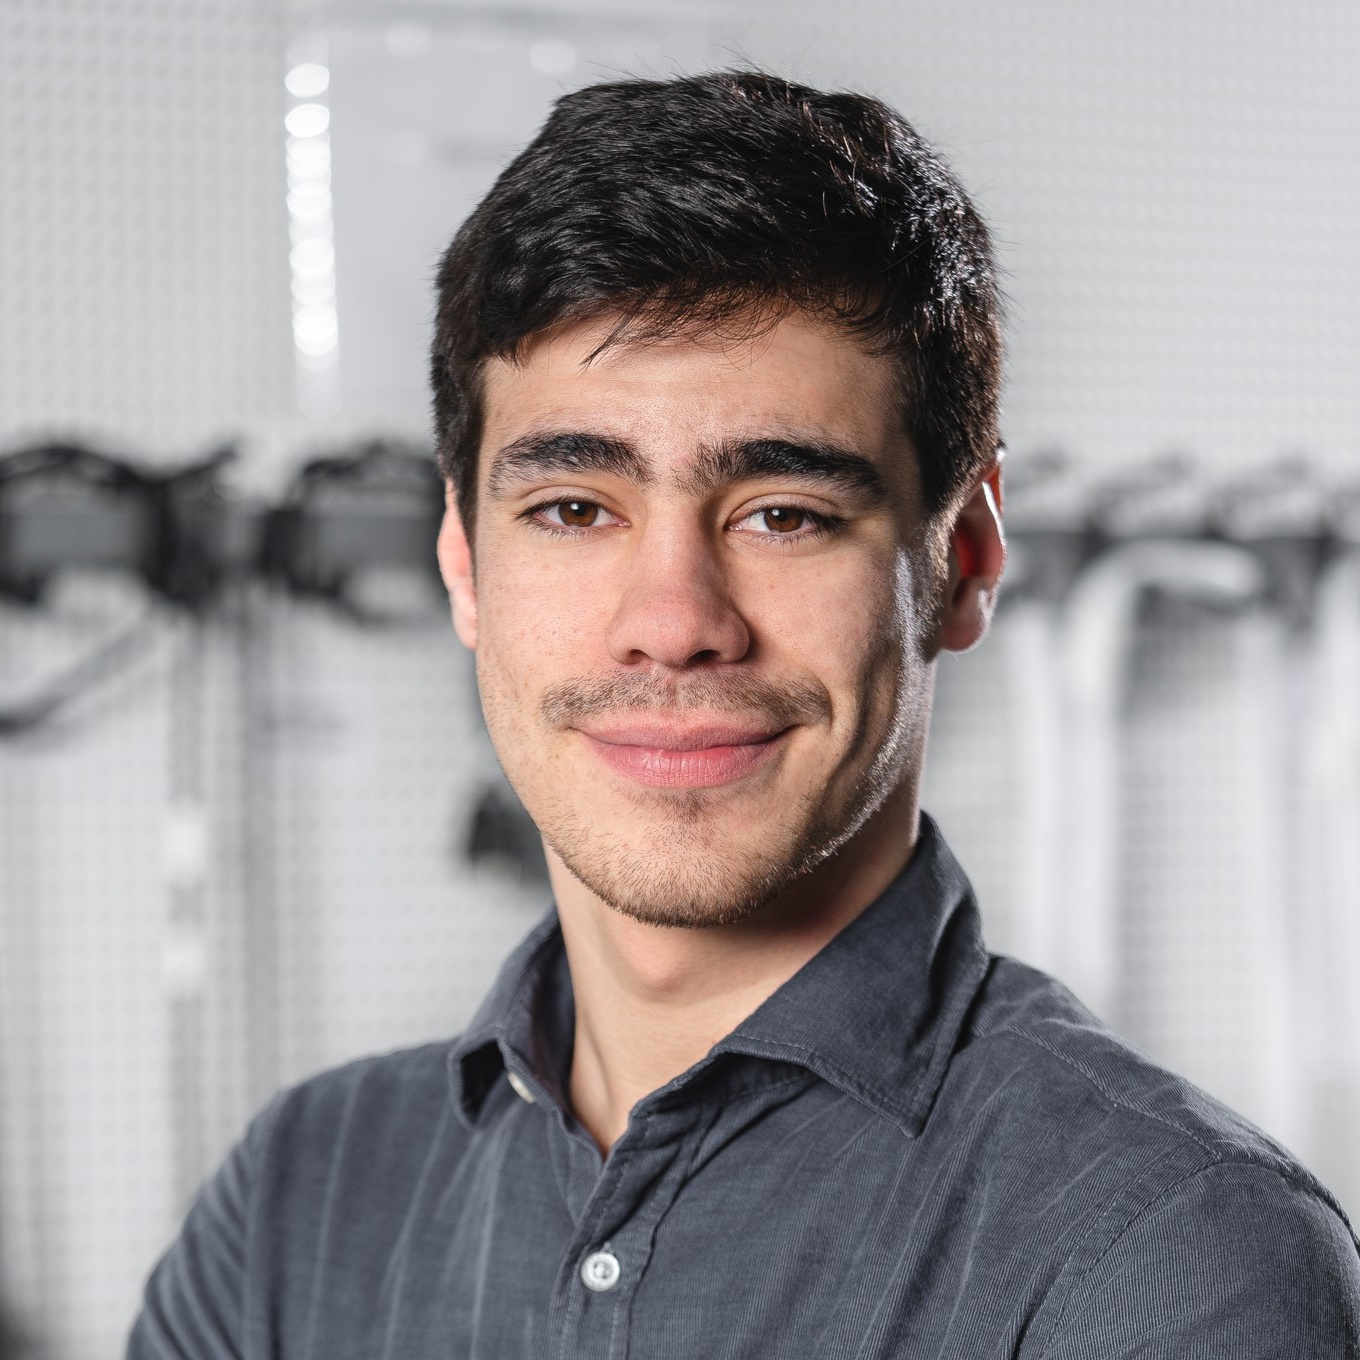
\includegraphics[width=\linewidth]{portrait.jpg}
		% \fcolorbox{white}{white}{\begin{minipage}[c][1.5cm][c]{1\mpwidth}
		% 		\LARGE{\textbf{\textcolor{maincol}{David Munoz-Tord}}} 
				% \normalsize{ \textcolor{maincol} {} }
			% \end{minipage}}

		%---------------------------------------------------------------------------------------
		%	META SKILLS
		%----------------------------------------------------------------------------------------
		
		
		\cvsection{Senior R Developer}

						\icontext{map-marker}{16}{Geneva, Switzerland}\\[0pt]
								\icontext{envelope}{16}{david.munoztord@mailbox.org}\\[0pt]
								\iconhref{home}{16}{david-munoztord.online}{https://munoztd0.github.io/homepage/}\\[0pt]
								\iconhref{github}{16}{munozt0}{https://github.com/munoztd0}\\[0pt]
								\iconhref{linkedin}{16}{david-munoz-tord}{https://www.linkedin.com/in/david-munoz-tord-409639150/}\\[0pt]
						
		\cvsection{Skills}

						\cvskill{R}{10 yrs.}{1} \\[0pt]
								\cvskill{Python}{5 yrs.}{0.8} \\[0pt]
								\cvskill{Bash}{7 yrs.}{0.9} \\[0pt]
								\cvskill{Docker}{5 yrs.}{0.8} \\[0pt]
								\cvskill{AWS (ECS / EC2)}{5 yrs.}{0.7} \\[0pt]
						
		\cvsection{Libraries}

						\icontext{caret-right}{12}{echarts, ggplot2, plotly, seaborn}\\[0pt]
								\icontext{caret-right}{12}{R Shiny, Dash, Streamlit}\\[0pt]
								\icontext{caret-right}{12}{tidyverse, data.table, dplyr}\\[0pt]
								\icontext{caret-right}{12}{TensorFlow, Keras, PyTorch,
Scikit-learn}\\[0pt]
								\icontext{caret-right}{12}{Rstan, brms, JAGS}\\[0pt]
								\icontext{caret-right}{12}{H2O, XGBoost, LightGBM}\\[0pt]
						
		\cvsection{Tools/Frameworks}

						\icontext{caret-right}{12}{Git / BASH}\\[0pt]
								\icontext{caret-right}{12}{Powershell}\\[0pt]
								\icontext{caret-right}{12}{Docker}\\[0pt]
								\icontext{caret-right}{12}{CI/CD}\\[0pt]
								\icontext{caret-right}{12}{AWS, Azure}\\[0pt]
								\icontext{caret-right}{12}{Posit}\\[0pt]
						
		\cvsection{Languages}

						\cvskill{French}{Native}{1} \\[0pt]
								\cvskill{Spanish}{Native}{1} \\[0pt]
								\cvskill{English}{Fluent}{1} \\[0pt]
								\cvskill{German}{Passive}{0.4} \\[0pt]
								\cvskill{Italian}{Professional}{0.8} \\[0pt]
						
	\end{leftcolumn}

	\begin{rightcolumn}
		\cvsection{Summary} \vspace{4pt}

\cvtext{%
Senior R Developer specialized in R data platforms and cloud-based
analytical infrastructures.\\
Proven experience designing, deploying, and maintaining containerized
environments for regulated sectors including banking and
pharmaceuticals. Strong track record in industrializing R workflows for
non-technical users, ensuring platform reliability, automation,
documentation, and operational continuity. Experienced with AWS
infrastructures, Posit Server ecosystems, and CI/CD workflows.}

\cvsection{Experience} \vspace{4pt}

\cvevent{02/2025 - Present}{Senior R Developer}{Johnson & Johnson}

\begin{itemize}
\tightlist
\item
  -- Designed and maintained containerized R platforms (Docker) for
  Posit Server ecosystems and pharma applications
\item
  -- Leading open-source R package development to accelerate insights
  generation in clinical research settings
\item
  -- Provided platform support, automation, documentation, and incident
  handling in regulated environments
\end{itemize}

\cvtext{%
}

\cvsection{Experience} \vspace{4pt}

\cvevent{01/2024 - 02/2025}{Data Science Consultant}{Freelancer - Pharmaceutical \\& Tech Sectors}

\begin{itemize}
\tightlist
\item
  -- Developed data infrastructure solutions for multiple clients,
  implementing process automation and cloud-based data management
  systems
\item
  -- Built and operated cloud-based analytical infrastructures on AWS
\item
  -- Conducted complex data analysis and predictive modeling across
  diverse industry domains, including healthcare and financial
  technology
\end{itemize}

\cvevent{04/2022 - 01/2024}{R Developer / Data Scientist}{FlowBank}

\begin{itemize}
\tightlist
\item
  -- Architected and operated production-grade analytics platforms based
  on R Shiny, Docker, and AWS
\item
  -- Maintained containerized machine learning pipelines for fraud
  detection and risk modeling
\item
  -- Managed internal data platforms used by data science teams,
  including job scheduling and user support
\item
  -- Collaborated closely with security and compliance teams in a
  regulated banking environment
\end{itemize}

\cvtext{%
}

\cvevent{09/2020 - 01/2022}{Lecturer in Biostatistics}{University of Geneva}

\begin{itemize}
\tightlist
\item
  -- Delivered statistics courses and practical workshops in R and
  Python
\item
  -- Produced and maintained teaching material and documentation for
  students
\end{itemize}

\cvtext{%
}

\cvevent{03/2020 - 01/2022}{Research Scientist}{Novo Nordisk - Campus Biotech, Switzerland}

\begin{itemize}
\tightlist
\item
  -- Developed large-scale data processing pipelines for clinical and
  neuroimaging data
\item
  -- Applied advanced Bayesian statistical modeling and machine learning
  techniques
\item
  -- Collaborated with international research teams and maintained
  rigorous data governance standards
\end{itemize}

\cvsection{Projects} \vspace{4pt}

\cvtext{%
See my \href{https://github.com/munoztd0}{\underline{github profile}}
for a more comprehensive list of open source projects.}

\cvsection{Publications} \vspace{4pt}

\cvtext{%
See my
\href{https://github.com/munoztd0/publications/tree/master}{\underline{publications pages}}
for a comprehensive list my scientific publications.}
			\end{rightcolumn}
\end{paracol}


\end{document}
